\documentclass[11pt,a4paper]{report}

\usepackage[utf8]{inputenc}
\usepackage[T1]{fontenc}
\usepackage[french]{babel}
\usepackage{geometry}
\usepackage{hyperref}
\usepackage{listings}
\usepackage{xcolor}
\usepackage{enumitem}
\usepackage{tabularx}
\usepackage{longtable}
\usepackage{booktabs}
\usepackage{fancyhdr}
\usepackage{tikz}
\usetikzlibrary{arrows.meta, positioning, fit, backgrounds}
\usepackage{titlesec}
\usepackage{graphicx}

\geometry{margin=2.5cm}

\definecolor{codegray}{rgb}{0.95,0.95,0.95}
\definecolor{fanteal}{RGB}{0,121,107}
\definecolor{fannavy}{RGB}{20,30,60}

\lstset{
  backgroundcolor=\color{codegray},
  basicstyle=\ttfamily\small,
  breaklines=true,
  frame=single,
  columns=fullflexible,
  showstringspaces=false,
  keywordstyle=\color{fanteal}\bfseries,
  commentstyle=\itshape\color{gray},
  literate={é}{{\'e}}1 {è}{{\`e}}1 {à}{{\`a}}1 {ù}{{\`u}}1 {ç}{{\c{c}}}1 {ê}{{\^e}}1 {î}{{\^i}}1 {ô}{{\^o}}1
}

\newcommand{\code}[1]{\lstinline{#1}}

\setlength{\headheight}{14.5pt}
\pagestyle{fancy}
\fancyhf{}
\fancyhead[L]{HUGO PRADIER}
\fancyhead[R]{DOSSIER PROJET}
\fancyfoot[C]{\thepage}
\renewcommand{\headrulewidth}{0.4pt}

\titleformat{\chapter}[hang]{\normalfont\Large\bfseries\color{fannavy}}{\thechapter.}{0.5em}{}

\hypersetup{
  colorlinks=true,
  linkcolor=fanteal,
  urlcolor=fanteal,
  citecolor=fanteal,
  pdftitle={FanFlight -- Dossier projet},
  pdfauthor={Hugo Pradier}
}

\title{
  \vspace{-2cm}
  {\Large DOSSIER PROJET}\\[0.3cm]
  {\large Cursus Data Engineer}\\[0.1cm]
  {\large RNCP38919}\\[1.2cm]
  {\Huge \bfseries \color{fannavy} Projet FanFlight}\\[0.4cm]
  {\large Plateforme de recherche de vols pour la Coupe du Monde 2026}\\[2cm]
  {\large Hugo PRADIER}\\[0.2cm]
  {\normalsize Projet réalisé avec Hugo Jacquit, Daniel Kouacou et Emy Regna}\\[0.6cm]
  {\normalsize Promotion 2025--2026}\\[0.1cm]
  {\normalsize Liora -- Certification DataScientest}
}
\author{}
\date{\today}

\begin{document}

\begin{titlepage}
\maketitle
\thispagestyle{empty}
\end{titlepage}

\pagenumbering{arabic}

\chapter*{Remerciements}
\addcontentsline{toc}{chapter}{Remerciements}

Je tiens à exprimer ma sincère gratitude envers tous ceux qui ont contribué à la réussite du projet FanFlight et à l'accomplissement de ma formation Data Engineer chez Liora, certifiée par DataScientest.

Mes remerciements s'adressent en premier lieu à Dan Cohen, notre mentor projet, pour son accompagnement, sa disponibilité et ses conseils techniques qui nous ont permis de faire les bons choix d'architecture au bon moment, en particulier sur les questions de coût et de robustesse du pipeline de données.

Je remercie également l'équipe pédagogique de Liora et de DataScientest pour la qualité de la formation et son accompagnement tout au long du cursus Data Engineer (RNCP38919).

Ma gratitude va tout particulièrement à mes coéquipiers, Hugo Jacquit, Daniel Kouacou et Emy Regna, avec qui ce projet a été mené du premier commit jusqu'à la mise en production. Malgré une équipe répartie sur toute la France et des emplois du temps contraints par nos alternances respectives, nous avons su maintenir une dynamique de travail collective sur la durée du projet -- une réussite en elle-même. Hugo Jacquit a posé les fondations du backend et du pipeline Spark ; Daniel Kouacou a poussé le projet au-delà de son périmètre initial en y intégrant un volet complet de machine learning ; Emy Regna a conçu et mis en place l'ensemble de la chaîne d'observabilité du projet.

Enfin, je remercie la communauté open-source (FastAPI, Apache Spark, PostgreSQL, Next.js, MLflow) dont la documentation et les forums ont été des ressources précieuses pour surmonter les obstacles techniques rencontrés.

\tableofcontents

\chapter{Introduction}

\section*{Accroche}
\addcontentsline{toc}{section}{Accroche}

En 2026, la Coupe du Monde de football réunit pour la première fois 48 équipes et un nombre record de 104 matchs, répartis dans 16 villes hôtes à travers trois pays -- les États-Unis, le Canada et le Mexique. Pour des millions de supporters, suivre son équipe favorite ne se limite plus à un aller-retour vers un stade voisin : cela implique de recouper un calendrier sportif dense avec une offre aérienne éclatée entre des dizaines de villes de départ et d'arrivée possibles, sur un continent entier. Or, aucun outil ne relie nativement ces deux mondes : le calendrier des matchs d'un côté, la disponibilité et le prix des vols de l'autre.

\section*{Contexte et enjeux}
\addcontentsline{toc}{section}{Contexte et enjeux}

Planifier un déplacement autour d'un match de Coupe du Monde suppose aujourd'hui de jongler entre plusieurs sources : le calendrier officiel de la compétition, des moteurs de recherche de vols génériques, et une vérification manuelle de la cohérence des dates. Cette fragmentation de l'information ralentit la décision et complique l'expérience du supporter, en particulier lorsqu'il doit comparer plusieurs villes de départ ou plusieurs matchs.

Du point de vue technique, connecter ces deux mondes pose un problème d'ingénierie de données classique mais exigeant : il faut collecter une donnée sportive stable (calendrier, équipes, villes hôtes) et une donnée de vol volatile et coûteuse à interroger (les fournisseurs de données de vol facturent chaque requête), les stocker dans un modèle cohérent, les transformer de façon fiable et industrialisable, puis les exposer à une interface utilisateur simple -- tout en maîtrisant un budget d'appels API et une infrastructure d'hébergement limités.

C'est ce double enjeu -- rendre accessible une information aujourd'hui fragmentée, tout en construisant un pipeline de données robuste et économiquement soutenable -- qui a motivé le choix du projet FanFlight comme projet fil rouge de notre cursus Data Engineer.

\section*{Définition des termes clés}
\addcontentsline{toc}{section}{Définition des termes clés}

\begin{description}[leftmargin=0cm, style=nextline]
\item[API (Application Programming Interface)] Interface permettant à deux applications de communiquer. FastAPI expose une API REST consommée par le frontend Next.js de FanFlight.
\item[BTS (Bureau of Transportation Statistics)] Agence fédérale américaine publiant des statistiques de ponctualité des vols domestiques. Utilisée dans l'extension machine learning de FanFlight comme source d'entraînement réelle.
\item[CI/CD (Continuous Integration / Continuous Deployment)] Pratique consistant à automatiser la construction, la vérification et le déploiement du code. GitHub Actions orchestre ce cycle pour FanFlight.
\item[Conteneur (Docker)] Unité logicielle packageant du code et ses dépendances pour une exécution reproductible. Chaque composant de FanFlight (frontend, API, Spark, base de données) est conteneurisé.
\item[Data Warehouse / Schéma en étoile] Modélisation de données organisée autour de tables de faits (\code{FACT_FLIGHT}, \code{FACT_MATCHS}) reliées à des tables de dimensions (\code{DIM_CITY}, \code{DIM_AIRPORT}, \code{DIM_TEAM}). Modèle retenu pour la base PostgreSQL de FanFlight.
\item[Docker Hub] Registre public d'images Docker. Les images de FanFlight y sont publiées sous le namespace \code{tezzosyris666}.
\item[Drift (dérive de données)] Évolution statistique des données en production par rapport aux données d'entraînement d'un modèle. Surveillée dans FanFlight via des tests PSI et Kolmogorov-Smirnov.
\item[ETL (Extract, Transform, Load)] Processus d'extraction, de transformation et de chargement de données. Implémenté par le pipeline Spark de FanFlight, qui transforme les réponses brutes de l'API de vols en enregistrements exploitables.
\item[Event-driven architecture (architecture événementielle)] Architecture où un traitement est déclenché par un événement plutôt que par un ordonnancement périodique. Le pipeline Spark de FanFlight est déclenché par une notification PostgreSQL, pas par une tâche planifiée (cron).
\item[FastAPI] Framework Python pour construire des API REST avec validation automatique des données et documentation OpenAPI générée. Framework backend de FanFlight.
\item[GitHub Actions] Plateforme d'intégration et de déploiement continu intégrée à GitHub. Orchestre la construction des images Docker et le déploiement de FanFlight.
\item[Grafana] Plateforme open-source de visualisation de métriques sous forme de tableaux de bord. Utilisée par FanFlight pour restituer les métriques collectées par Prometheus.
\item[IATA] Code à trois lettres identifiant un aéroport (ex. \code{JFK}, \code{LAX}). Utilisé comme clé de correspondance entre villes et aéroports dans FanFlight.
\item[JSONB] Type de colonne PostgreSQL stockant du JSON de façon binaire et indexable. Utilisé par FanFlight pour la table d'atterrissage \code{FLIGHTS_RAW}, qui conserve les réponses brutes de l'API de vols avant leur transformation.
\item[LISTEN/NOTIFY] Mécanisme natif de PostgreSQL permettant à un processus de notifier des événements à des processus abonnés. Utilisé par FanFlight pour déclencher le pipeline Spark dès qu'une nouvelle donnée de vol brute est insérée.
\item[MLflow] Plateforme open-source de suivi d'expériences et de registre de modèles de machine learning. Utilisée dans l'extension ML de FanFlight pour comparer et versionner les modèles de prédiction de retard.
\item[MLOps] Ensemble de pratiques visant à industrialiser le cycle de vie des modèles de machine learning (entraînement, déploiement, monitoring). Illustré dans FanFlight par le registre de modèles MLflow et le monitoring de dérive.
\item[Model Registry] Composant de MLflow qui versionne les modèles entraînés et gère leur promotion vers un statut « Production ». Utilisé pour le modèle \code{flight_delay_xgboost} de FanFlight.
\item[Next.js] Framework React pour construire des applications web. Framework du frontend de FanFlight (version 16, App Router).
\item[Open-Meteo] API météorologique gratuite et open-data. Utilisée dans FanFlight pour enrichir les données de vol avec des conditions météorologiques réelles ou prévisionnelles.
\item[PostgreSQL] Système de gestion de base de données relationnelle open-source. Base de données centrale de FanFlight, épinglée en version 17.
\item[Prometheus] Système open-source de collecte et de stockage de métriques temporelles, interrogé périodiquement (\emph{scraping}) auprès de ses cibles. Collecteur central de la chaîne d'observabilité de FanFlight.
\item[PySpark / Apache Spark] Framework de traitement de données distribué et son API Python. Moteur du pipeline ETL de FanFlight.
\item[RGPD] Règlement Général sur la Protection des Données. FanFlight ne traite aucune donnée personnelle identifiante : la seule donnée utilisateur est une ville de départ sélectionnée dans une liste fermée.
\item[RNCP] Répertoire National des Certifications Professionnelles. RNCP38919 « Data engineer » est le référentiel de certification du présent cursus.
\item[SerpAPI] Service tiers exposant, entre autres, les résultats de recherche de vols de Google Flights sous forme d'API. Source de données de vol externe de FanFlight, facturée à la requête.
\item[Surrogate key (clé de substitution)] Identifiant technique généré (ici par hachage MD5) plutôt qu'extrait directement de la donnée source. Utilisée par FanFlight (\code{journey_sk}, \code{flight_sk}) pour garantir l'idempotence des insertions.
\item[Watchtower] Service qui surveille un registre Docker et met à jour automatiquement les conteneurs en production dès qu'une nouvelle image est disponible. Utilisé pour le déploiement continu de FanFlight sur l'instance EC2 de production.
\item[XGBoost] Bibliothèque de gradient boosting sur arbres de décision, très utilisée sur données tabulaires. Modèle retenu pour la prédiction de retard de vol dans l'extension ML de FanFlight.
\end{description}

\section*{Présentation du projet FanFlight}
\addcontentsline{toc}{section}{Présentation du projet FanFlight}

FanFlight est une application web qui permet à un supporter de choisir sa ville de départ, de consulter les matchs de la Coupe du Monde 2026, puis de visualiser des propositions de vols cohérentes avec le calendrier du match sélectionné. Le parcours utilisateur se déroule en trois étapes guidées : sélection de la ville de départ, sélection du match, puis consultation des vols proposés. La version livrée couvre le calendrier de la phase de groupes de l'édition 2026 ; l'extension aux phases finales de la compétition est identifiée comme un axe d'évolution (cf. section~\ref{sec:preconisations}).

Voici une capture d'écran de l'écran d'accueil de l'application FanFlight.

\begin{figure}[h]
\centering
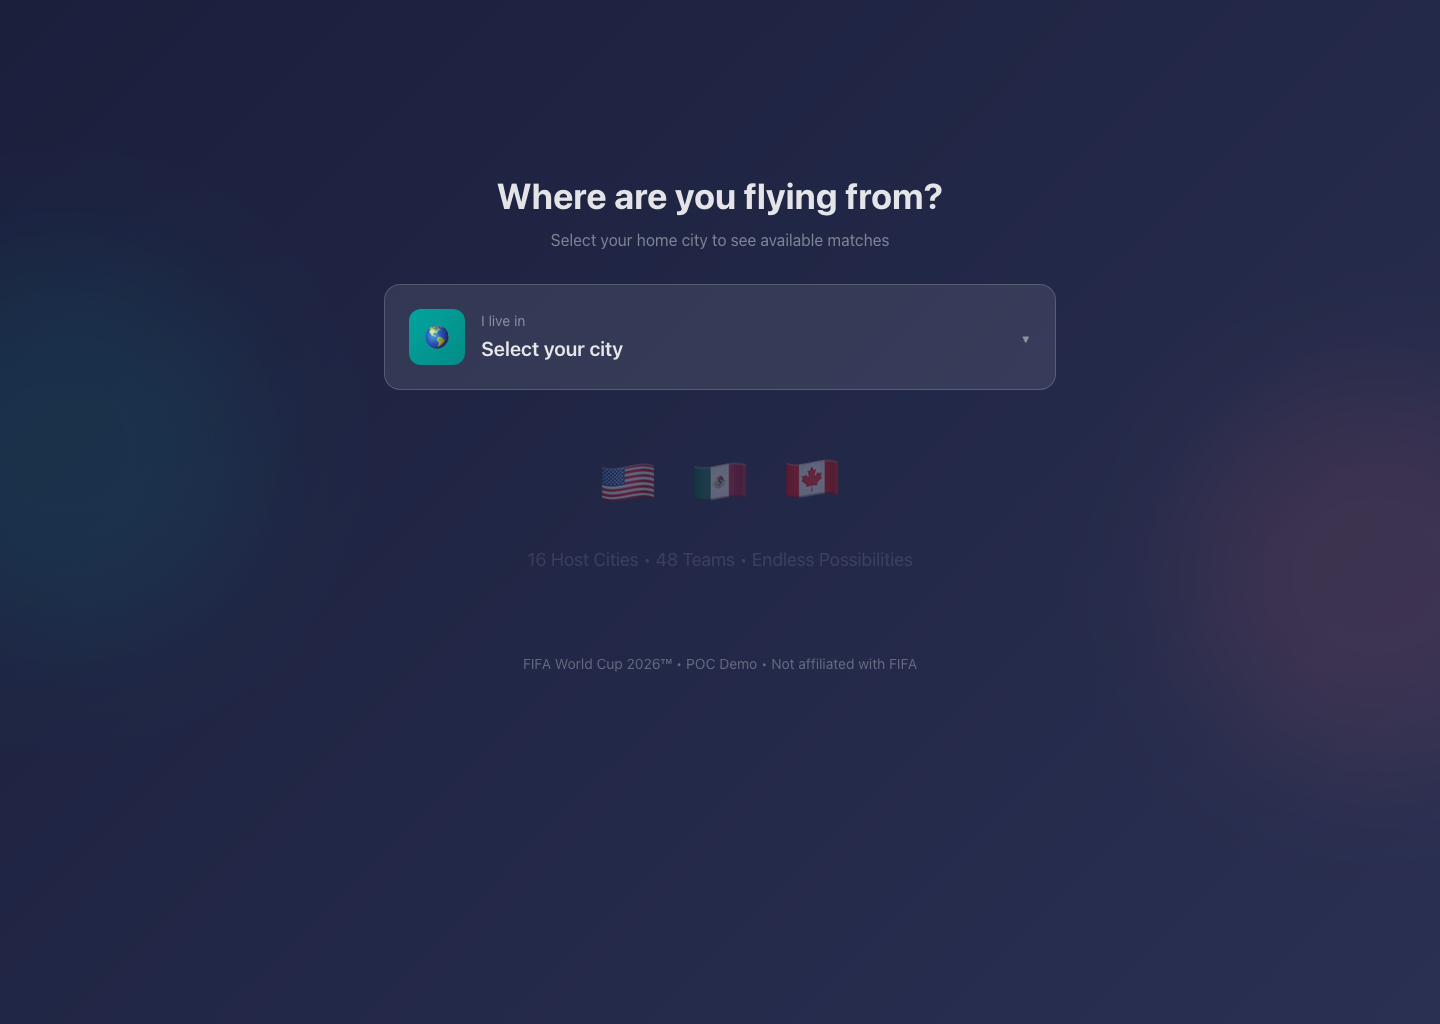
\includegraphics[width=0.75\textwidth]{img/app-city-select.png}
\caption{Écran d'accueil de FanFlight -- sélection de la ville de départ}
\label{fig:app-accueil}
\end{figure}

Le projet a été développé dans le cadre de notre formation Data Engineer chez Liora (certification DataScientest, RNCP38919) par une équipe de quatre personnes -- Hugo Pradier, Hugo Jacquit, Daniel Kouacou et Emy Regna -- répartie sur l'ensemble du territoire français et conciliant ce projet fil rouge avec nos alternances respectives. Contrairement à un scénario où l'équipe se serait délitée en cours de route, notre défi a été inverse : rester coordonnés à distance sur la durée du projet malgré ces contraintes (cf. section « Contraintes du projet »).

\begin{figure}[h]
\centering
\begin{tabular}{cccc}

\includegraphics[width=2.6cm]{img/1732648926225.jpeg} &
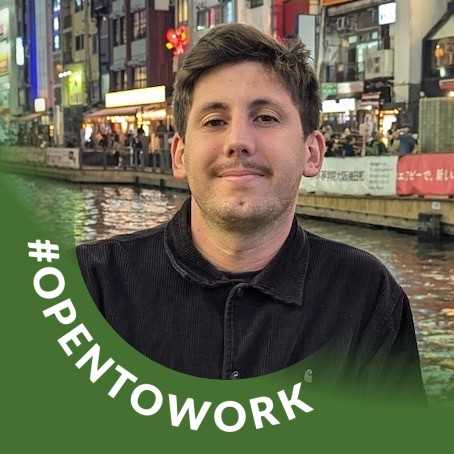
\includegraphics[width=2.6cm]{img/1781626577471.jpeg} &

\includegraphics[width=2.6cm]{img/1679003524013.jpeg} &
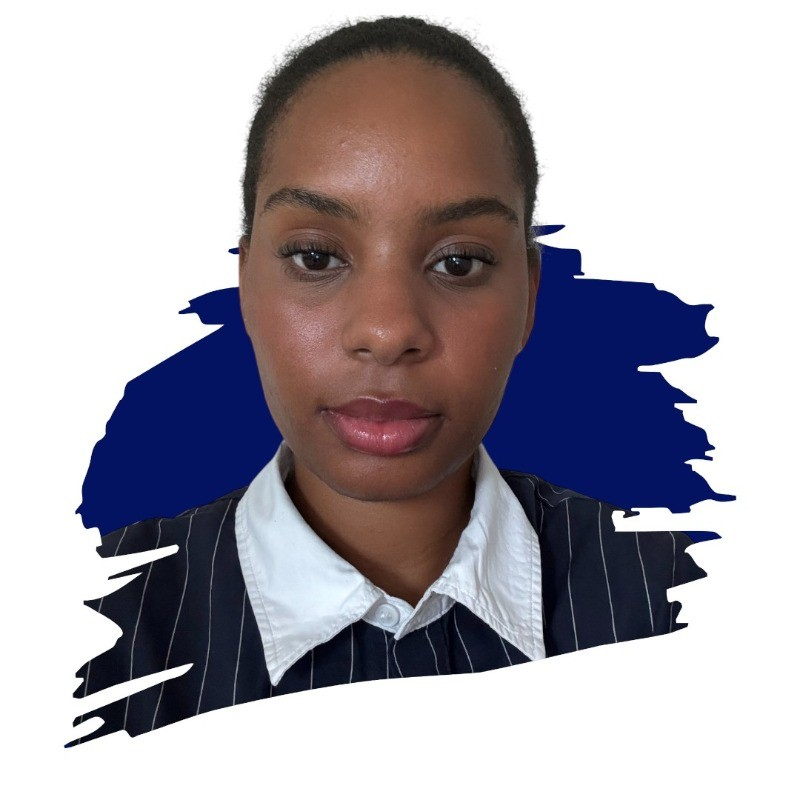
\includegraphics[width=2.6cm]{img/1739468289142.jpeg} \\
\textbf{Hugo Pradier} & \textbf{Hugo Jacquit} & \textbf{Daniel Kouacou} & \textbf{Emy Regna} \\
\footnotesize Infrastructure, pipeline, & \footnotesize Backend, pipeline Spark, & \footnotesize Extension machine & \footnotesize Observabilité \\
\footnotesize déploiement & \footnotesize base de données & \footnotesize learning & \footnotesize (Prometheus/Grafana) \\
\end{tabular}
\caption{L'équipe du projet FanFlight}
\label{fig:equipe}
\end{figure}

\section*{Environnement technique et architecture}
\addcontentsline{toc}{section}{Environnement technique et architecture}

FanFlight repose sur une architecture conteneurisée orchestrée par Docker Compose, structurée autour des technologies suivantes :

\begin{itemize}
  \item \textbf{Frontend} : Next.js 16 (App Router) / React 19 / Tailwind CSS 4 / framer-motion
  \item \textbf{Backend} : FastAPI (Python), API REST documentée automatiquement (OpenAPI)
  \item \textbf{Base de données} : PostgreSQL 17, schéma en étoile hybride relationnel / JSONB
  \item \textbf{Pipeline de données} : Apache Spark (PySpark), déclenché par événements PostgreSQL (\code{LISTEN}/\code{NOTIFY})
  \item \textbf{Source de données externe} : SerpAPI (moteur \code{google_flights})
  \item \textbf{Extension Machine Learning} : XGBoost / PyTorch, suivi et registre via MLflow
  \item \textbf{Observabilité} : Prometheus, Grafana, Blackbox Exporter, node-exporter, cAdvisor, postgres-exporter
  \item \textbf{Conteneurisation} : Docker, images publiées sur Docker Hub (namespace \code{tezzosyris666})
  \item \textbf{CI/CD} : GitHub Actions (build, push, déploiement SSH)
  \item \textbf{Déploiement continu} : Watchtower (mise à jour automatique des conteneurs en production)
  \item \textbf{Hébergement de production} : instance AWS EC2, fournie par notre école en cours de projet
\end{itemize}

La figure~\ref{fig:archi} synthétise les flux entre ces composants.

\begin{figure}[h]
\centering
\begin{tikzpicture}[
  box/.style={rectangle, rounded corners, draw=fannavy, fill=fannavy!8, minimum width=2.8cm, minimum height=1.1cm, align=center, font=\small},
  ext/.style={rectangle, rounded corners, draw=gray, fill=gray!10, minimum width=2.8cm, minimum height=1.1cm, align=center, font=\small},
  arr/.style={-Latex, thick},
  lbl/.style={font=\tiny, fill=white, inner sep=1pt}
]
\node[box] (front) at (0,3.6) {Frontend\\Next.js};
\node[box] (api) at (5,3.6) {API\\FastAPI};
\node[ext] (serp) at (10.4,3.6) {SerpAPI\\(google\_flights)};
\node[box] (db) at (5,-0.6) {PostgreSQL\\(star schema + JSONB)};
\node[box] (spark) at (10.4,-0.6) {Spark\\(master/worker)};

\draw[arr] (front) -- node[lbl, above] {fetch /api/*} (api);
\draw[arr] (api) -- node[lbl, pos=0.62] {si cache vide} (serp);
\draw[arr] (api) edge[bend left=18] node[lbl, pos=0.25] {lecture cache} (db);
\draw[arr] (api) edge[bend right=18] node[lbl, pos=0.78] {insertion JSON brut} (db);
\draw[arr] (db) edge[bend left=15] node[lbl, pos=0.5] {LISTEN/NOTIFY} (spark);
\draw[arr] (spark) edge[bend left=15] node[lbl, pos=0.5] {STG\_FLIGHT $\to$ FACT\_FLIGHT} (db);
\end{tikzpicture}
\caption{Architecture applicative et flux de données de FanFlight}
\label{fig:archi}
\end{figure}

\section*{Annonce du plan}
\addcontentsline{toc}{section}{Annonce du plan}

Ce dossier présente d'abord les compétences du référentiel RNCP38919 mobilisées par le projet FanFlight. Nous détaillerons ensuite le cahier des charges du projet, puis la démarche et les outils utilisés pour le mener à bien en équipe distribuée. La présentation de nos réalisations techniques concrètes sera suivie d'une analyse d'une problématique de recherche rencontrée en cours de projet -- le contrôle du coût des appels à l'API externe de vols. Nous conclurons par une synthèse des difficultés rencontrées, des bénéfices tirés du projet, et des perspectives d'évolution.

\chapter{Compétences du référentiel RNCP38919 couvertes par le projet}

Le titre « Data engineer » (RNCP38919, niveau 7, certificateur DataScientest) est structuré en quatre blocs de compétences (BC01 à BC04). Le projet FanFlight a été construit pour couvrir l'intégralité de ces blocs et en démontrer la maîtrise de manière concrète.

\section{BC01 -- Concevoir un projet d'architecture technique de gestion de données}

\subsection{Identifier les besoins en architecture de gestion de données}

Le besoin a été formalisé à partir d'un constat simple : un supporter de la Coupe du Monde 2026 doit croiser manuellement deux sources d'information (calendrier des matchs et offres de vols) sans qu'aucun outil ne les relie. Nous avons analysé le flux de données nécessaire -- données sportives stables (équipes, villes hôtes, calendrier) et données de vol volatiles et coûteuses à obtenir (SerpAPI) -- pour valider l'opportunité et le périmètre technique du projet.

\subsection{Élaborer et exercer un système de veille technologique et réglementaire}

Notre veille technique et réglementaire a porté sur plusieurs axes structurants :
\begin{itemize}
  \item comparaison de fournisseurs de données de vol (API dédiées vs scraping) et sélection de SerpAPI pour son accès à Google Flights ;
  \item évaluation d'une architecture de traitement par lot (cron) contre une architecture événementielle -- retenue pour limiter la latence perçue côté utilisateur ;
  \item étude des mécanismes natifs PostgreSQL (\code{LISTEN}/\code{NOTIFY}) comme alternative légère à une file de messages (Kafka, RabbitMQ), jugée disproportionnée pour le volume et le budget du projet ;
  \item veille sur les pratiques de MLOps (MLflow, model registry, monitoring de dérive) pour l'extension machine learning ;
  \item veille réglementaire sur la protection des données (RGPD), pour vérifier qu'un traitement ne collectant aucune donnée personnelle identifiante restait hors du champ des obligations les plus contraignantes, et sur les recommandations relatives à l'explicabilité des modèles de scoring, qui ont motivé le recours à SHAP pour documenter les prédictions du modèle de retard (cf. section~\ref{sec:ml}).
\end{itemize}

\subsection{Exploiter la veille au sein de l'équipe}

Les arbitrages techniques ont été partagés et discutés entre les quatre membres de l'équipe et avec notre mentor Dan Cohen, malgré l'absence de coprésence physique. Les décisions d'architecture (schéma en étoile, pipeline événementiel, stratégie de cache) ont fait l'objet de revues de code via des \emph{pull requests} sur GitHub avant fusion sur la branche principale.

\subsection{Définir le périmètre du projet}

Le périmètre a été formalisé autour de : (1) un socle de données de référence figées pour l'édition 2026 (équipes, villes hôtes, calendrier des matchs de phase de groupes -- l'extension aux phases finales étant un axe d'évolution identifié, cf. section~\ref{sec:preconisations}), (2) une couche dynamique de vols alimentée à la demande, (3) une interface de consultation. Les enjeux réglementaires ont été jugés limités : FanFlight ne collecte aucune donnée personnelle identifiante, la seule saisie utilisateur étant une ville de départ choisie dans une liste fermée. L'enjeu principal identifié était économique : le coût par appel de l'API externe de vols imposait de concevoir le système pour minimiser les requêtes redondantes dès la conception (cf. chapitre~\ref{chap:recherche}). Ce même arbitrage a aussi guidé un choix à faible empreinte : privilégier les mécanismes déjà natifs de PostgreSQL (\code{LISTEN}/\code{NOTIFY}) plutôt que d'ajouter un service dédié supplémentaire (file de messages, cache Redis) limite le nombre de conteneurs actifs en permanence, et donc la consommation de ressources de l'infrastructure -- un objectif de sobriété numérique qui rejoignait naturellement la contrainte budgétaire.

\subsection{Émettre des recommandations}

Les choix d'architecture ont été présentés et défendus au sein de l'équipe puis auprès de notre mentor : modèle de données en étoile plutôt que documentaire, pipeline événementiel plutôt que batch, cache applicatif porté par PostgreSQL plutôt que par une brique dédiée (Redis) pour ne pas alourdir l'infrastructure à opérer par une petite équipe.

\section{BC02 -- Élaborer une architecture technique de gestion de données}

\subsection{Collecter les données structurées et non structurées}

FanFlight combine deux natures de données : des données structurées codées en dur pour l'édition 2026 (équipes, villes hôtes et leurs aéroports, calendrier des matchs, dans \code{load_static_data.py}) et des données semi-structurées collectées dynamiquement (réponses JSON de SerpAPI), stockées telles quelles avant transformation. Un référentiel externe (\code{airport-codes.csv}) est également mobilisé pour enrichir les aéroports inconnus au fil de l'utilisation.

\subsection{Élaborer des solutions de stockage}

Le stockage repose sur PostgreSQL, avec un modèle hybride :
\begin{itemize}
  \item un schéma en étoile relationnel classique -- tables de dimensions \code{DIM_CITY}, \code{DIM_AIRPORT}, \code{DIM_TEAM} et tables de faits \code{FACT_MATCHS}, \code{FACT_FLIGHT} ;
  \item une table d'atterrissage semi-structurée \code{FLIGHTS_RAW} en colonne \code{JSONB}, qui conserve la réponse brute de l'API externe avant sa transformation, avec un indicateur \code{processed} servant de suivi (\emph{watermark}) du pipeline.
\end{itemize}

\subsection{Concevoir les procédures d'extraction, de transformation et de stockage}

Le pipeline suit un schéma classique \emph{staging puis fusion} : les données brutes sont extraites de la table d'atterrissage \code{FLIGHTS_RAW}, transformées par un job Spark dans une table de \emph{staging} (\code{STG_FLIGHT}), puis fusionnées de façon idempotente dans la table de faits finale (\code{FACT_FLIGHT}) via une clause \code{ON CONFLICT ... DO UPDATE}. Ce détail est développé au chapitre~\ref{chap:realisations}.

\subsection{Transformer les données en un format approprié}

La transformation Spark infère dynamiquement le schéma JSON de chaque réponse SerpAPI (\code{schema_of_json}), sépare les propositions « meilleurs vols » et « autres vols », éclate chaque itinéraire en segments de vol (\code{posexplode}), calcule des clés de substitution par hachage MD5 pour garantir l'unicité et l'idempotence, gère de façon défensive les champs optionnels (une correspondance -- \emph{layover} -- n'existe pas pour un vol direct), et déduplique les segments avant chargement.

\subsection{Analyser les données}

La qualité et la disponibilité des données sont évaluées à chaque requête : la fonction \code{check_flight_db} vérifie si un trajet aller valide existe déjà en base -- un vol reliant la ville de départ de l'utilisateur à la ville du match, dont l'arrivée se situe entre 3 jours avant le match et, au plus tard, 5 heures avant son coup d'envoi -- avant de déclencher un nouvel appel à l'API externe. Les résultats sont ensuite restitués à l'utilisateur final via l'interface de vols. À une échelle plus large, l'évaluation de la qualité des données a également été formalisée dans l'extension machine learning du projet, via des tests statistiques de dérive (indice PSI, test de Kolmogorov--Smirnov, cf. section~\ref{sec:ml}) dont les résultats ont vocation à être partagés avec l'équipe et notre mentor lors des points d'avancement.

\subsection{Automatiser les circuits de collecte, de traitement et de stockage}

L'ensemble du circuit est automatisé de bout en bout : une notification PostgreSQL déclenche automatiquement le job Spark, qui déclenche à son tour la fusion vers la table de faits et la mise à jour du statut de traitement -- sans intervention manuelle. Le script \code{entrypoint.sh} du conteneur API rejoue, à chaque démarrage, l'initialisation du schéma et le chargement des données de référence -- deux étapes rendues idempotentes par des clauses \code{ON CONFLICT}. Il exécute aussi systématiquement \code{replay_job.py}, qui réinjecte les réponses SerpAPI déjà sauvegardées sur disque : cette dernière étape n'est, elle, pas idempotente et déclenche un nouveau job Spark à chaque redémarrage du conteneur (cf. chapitre~\ref{chap:recherche} et section~\ref{sec:preconisations}).

\subsection{Développer un algorithme d'intelligence artificielle}

Un algorithme de classification binaire (probabilité de retard de vol) a été développé par Daniel Kouacou sur une branche dédiée du projet, combinant des données réelles de ponctualité aérienne américaine (BTS) et des données météorologiques (Open-Meteo), avec deux modèles comparés (XGBoost et un réseau de neurones PyTorch). Ce travail est détaillé en section~\ref{sec:ml}.

\section{BC03 -- Déployer une solution d'analyse de données massives intégrant l'intelligence artificielle}

\subsection{Concevoir une interface de programmation}

L'API FastAPI constitue l'interface unique entre le frontend, la base de données et -- dans l'extension machine learning -- le modèle de prédiction. Elle expose des routes REST simples (\code{/api/matches}, \code{/api/teams}, \code{/api/cities}, \code{/api/flights/\{match\_id\}}) et bénéficie d'une documentation OpenAPI générée automatiquement par FastAPI.

\subsection{Conteneuriser les composants de l'architecture}

Chaque composant (frontend, API, Spark) dispose de son propre \code{Dockerfile} et de sa propre image, publiée sur Docker Hub. Ces images n'installent que les paquets système strictement nécessaires -- par exemple \code{gcc}/\code{libpq-dev} dans l'image Spark, requis pour compiler \code{psycopg2} (le pilote Python utilisé par \code{spark\_listener.py} et \code{stg\_to\_fact.py}), à ne pas confondre avec le pilote JDBC PostgreSQL utilisé par Spark lui-même, ajouté comme binaire préconstruit et ne nécessitant aucune compilation. L'accès aux registres et à l'infrastructure de production est protégé par une gestion de secrets : les identifiants Docker Hub et la clé SSH de déploiement sont stockés comme secrets GitHub Actions, jamais en clair dans le code versionné. Seule l'image frontend s'exécute toutefois avec un utilisateur non privilégié dédié ; les images API et Spark tournent encore avec un utilisateur root, ce qui constitue une piste de durcissement identifiée pour la suite du projet (cf. section~\ref{sec:preconisations}).

\subsection{Déployer le modèle dans un environnement de production}

Dans l'extension machine learning, le modèle est versionné et promu au statut « Production » via le registre de modèles MLflow, puis chargé par l'API à son démarrage (\emph{hook} \code{@app.on_event("startup")}) pour scorer chaque vol renvoyé par l'API en temps réel.

\subsection{Orchestrer les services de la solution}

Docker Compose orchestre l'ensemble des services : base de données, cluster Spark (\emph{master} et \emph{worker}), API, frontend, et -- pour l'extension ML -- serveur MLflow. Les dépendances de démarrage sont explicitées via des conditions \code{depends_on} (par exemple l'API n'accepte des requêtes qu'une fois la base de données déclarée saine par son \emph{healthcheck}).

\subsection{Contrôler la mise en production de la solution}

Un fichier \code{docker-compose.local.yml} permet de rejouer, en local, une configuration proche de la production (images pré-construites, mêmes variables d'environnement) avant tout déploiement réel. Le pipeline de déploiement inclut par ailleurs une étape de diagnostic automatique (relevé des journaux des conteneurs \code{postgres} et \code{backend\_api}) en cas d'échec du démarrage des services sur l'instance de production.

\subsection{Automatiser le déploiement de nouvelles versions et son monitoring}

Le déploiement continu repose sur GitHub Actions (construction et publication des images à chaque \emph{push} sur la branche principale) et sur Watchtower, qui surveille Docker Hub toutes les 60 secondes et met à jour automatiquement les conteneurs de production dès qu'une nouvelle image \code{latest} est disponible. Le monitoring de l'infrastructure elle-même est couvert par la chaîne d'observabilité développée par Emy Regna (Prometheus, Grafana, cf. section~\ref{sec:monitoring}), et le monitoring de l'évolution des données par un script de détection de dérive pour l'extension ML (\code{drift\_monitor.py}, tests PSI et Kolmogorov--Smirnov).

\section{BC04 -- Piloter un projet d'architecture technique de gestion de données}

\subsection{Définir la structure organisationnelle du projet}

Le projet a été structuré en quatre flux de travail répartis selon les affinités de chacun : Hugo Pradier sur l'infrastructure, l'intégration du pipeline de données et le déploiement ; Hugo Jacquit sur l'amorçage du backend, du pipeline Spark et de la base de données ; Daniel Kouacou sur l'extension machine learning ; Emy Regna sur la chaîne d'observabilité de l'infrastructure (Prometheus, Grafana). Cette organisation a dû composer avec une contrainte forte, détaillée au chapitre~\ref{chap:cahier} : une équipe répartie sur toute la France, chacun en alternance en entreprise en parallèle du projet.

\subsection{Encadrer le développement du projet}

Le développement a suivi une démarche itérative inspirée des pratiques agiles, adaptée à une équipe distribuée ne pouvant pas se caler sur des rituels synchrones quotidiens : le travail a été découpé en lots livrables et intégrables indépendamment (amorçage, socle backend/Spark/API, fiabilisation de la base, intégration ETL/frontend, durcissement du déploiement, extension machine learning -- cf. chapitre~\ref{chap:realisations} et section « Démarche technique »), chacun validé par une revue systématique de code avant fusion sur la branche principale -- trois de ces lots ont ainsi fait l'objet d'une fusion formelle par \emph{pull request}. Un accompagnement régulier de notre mentor Dan Cohen a complété ce cadre, avec un rôle proche de celui d'un \emph{product owner} : validation des choix d'architecture et priorisation des lots suivants. Le travail à distance a par ailleurs nécessité une discipline de communication asynchrone plus poussée qu'un travail en présentiel n'en aurait exigé.

\subsection{Gérer le budget du projet}

Deux postes de coût ont structuré les arbitrages du projet : le coût par requête de l'API externe de vols (SerpAPI), qui a directement orienté la conception du pipeline vers une architecture minimisant les appels redondants (cf. chapitre~\ref{chap:recherche}), et le coût d'hébergement de la production, initialement incertain, résolu lorsque notre école (Liora) a mis à notre disposition une instance AWS EC2 en fin de projet. Le suivi du premier poste a porté sur la conception même des requêtes envoyées à SerpAPI : chaque recherche interroge toutes les combinaisons d'aéroports possibles entre la ville de départ et la ville d'arrivée, sur les 3 jours précédant le match -- un facteur multiplicatif qu'il fallait garder à l'esprit pour ne déclencher ce coût qu'au moment d'un véritable cache manqué, jamais de façon spéculative.

\subsection{Communiquer l'avancement et les résultats du projet}

L'avancement a été communiqué régulièrement à notre mentor et synthétisé au fil de l'historique Git (structuration initiale, intégration backend/Spark/API, correctifs de base de données, intégration ETL/frontend, durcissement du déploiement), permettant un suivi transparent de la progression malgré le travail à distance.

\subsection{Évaluer la performance du projet}

La performance du pipeline a été évaluée sur des critères concrets : taux de réussite du cache de vols (proportion de requêtes servies directement depuis PostgreSQL sans nouvel appel à SerpAPI), respect du délai maximal de 90 secondes toléré pour un cycle complet d'enrichissement asynchrone, et -- pour le volet machine learning -- l'aire sous la courbe ROC (AUC) des modèles de prédiction de retard (0,728 pour XGBoost).

\subsection{Former les utilisateurs finaux de la solution}

Le plan d'accompagnement conçu pour les utilisateurs finaux de FanFlight repose sur le parcours lui-même : un assistant en trois étapes (ville, match, vols) où chaque écran ne présente que l'action suivante possible, pensé pour ne nécessiter aucune documentation externe. Ce parcours a été affiné au fil des points d'avancement avec notre mentor, qui a testé l'interface comme le ferait un utilisateur final et dont les retours ont permis d'ajuster son déroulé. Pour les utilisateurs techniques (contributeurs futurs, mainteneurs), la documentation OpenAPI générée automatiquement par FastAPI et les fichiers du dossier \code{documentation/} du dépôt jouent ce même rôle d'accompagnement.

\section{Synthèse de la couverture des compétences RNCP38919}

\begin{longtable}{p{2.6cm}p{4.2cm}p{6.8cm}}
\toprule
\textbf{Bloc} & \textbf{Compétence} & \textbf{Mise en œuvre dans FanFlight} \\
\midrule
\endhead
BC01 -- Concevoir & Identifier les besoins, veille, périmètre & Analyse du besoin supporter/vols, veille SerpAPI/architecture événementielle, périmètre formalisé en équipe \\
 & Émettre des recommandations & Choix défendus en équipe et avec le mentor (schéma en étoile, pipeline événementiel) \\
BC02 -- Élaborer & Collecter les données & Données statiques (équipes, villes, calendrier) + données SerpAPI dynamiques \\
 & Élaborer le stockage & PostgreSQL, schéma en étoile + table d'atterrissage JSONB \code{FLIGHTS_RAW} \\
 & Concevoir l'ETL & Pipeline Spark événementiel (staging $\to$ fusion upsert) \\
 & Transformer et analyser & Inférence de schéma, clés de substitution MD5, requêtes de disponibilité \\
 & Automatiser les circuits & \code{LISTEN}/\code{NOTIFY} + \code{entrypoint.sh} idempotent \\
 & Développer un algorithme d'IA & Modèle XGBoost / PyTorch de prédiction de retard (BTS + météo) \\
BC03 -- Déployer & Interface de programmation & API REST FastAPI, documentation OpenAPI \\
 & Conteneuriser & Docker par composant, images publiées sur Docker Hub \\
 & Déployer le modèle & Registre MLflow, chargement au démarrage de l'API \\
 & Orchestrer les services & Docker Compose (DB, Spark, API, frontend, MLflow) \\
 & Contrôler la mise en production & Compose « prod-like » local avant déploiement réel \\
 & Automatiser déploiement/monitoring & GitHub Actions + Watchtower + Prometheus/Grafana + \code{drift\_monitor.py} \\
BC04 -- Piloter & Structure organisationnelle & 4 rôles définis, équipe distribuée + alternances \\
 & Gérer le budget & Architecture pensée pour maîtriser le coût SerpAPI ; EC2 fourni par l'école \\
 & Évaluer la performance & Taux de cache, délai de pipeline, AUC du modèle ML \\
\bottomrule
\end{longtable}

\chapter{Cahier des charges du projet FanFlight}
\label{chap:cahier}

\section{Contexte et genèse du projet}

L'idée de FanFlight est née du constat que la Coupe du Monde 2026 -- première édition à 48 équipes, disputée dans 16 villes hôtes de trois pays différents -- allait démultiplier le besoin, pour les supporters, de déplacements complexes à planifier. Dans le cadre de notre formation Data Engineer chez Liora (certification DataScientest, RNCP38919), ce projet a été retenu comme projet fil rouge par une équipe de quatre personnes : Hugo Pradier, Hugo Jacquit, Daniel Kouacou et Emy Regna.

À la différence d'un projet d'équipe classique en présentiel, notre contexte de travail a été marqué dès le départ par une contrainte structurelle géographique et calendaire, détaillée ci-après (section « Contraintes du projet »).

\section{Objectifs du projet}

\textbf{Objectifs fonctionnels :}
\begin{itemize}
  \item permettre à un utilisateur de sélectionner une ville de départ et de consulter les matchs de la Coupe du Monde 2026 ;
  \item proposer, pour un match donné, des vols cohérents avec le calendrier (arrivée dans la ville du match jusqu'à 3 jours avant sa date, et au plus tard 5 heures avant son coup d'envoi) ;
  \item restituer ces informations dans une interface simple et guidée.
\end{itemize}

\textbf{Objectifs techniques et data engineering (prioritaires pour la certification) :}
\begin{itemize}
  \item concevoir un modèle de données combinant un référentiel stable et une donnée dynamique coûteuse à obtenir ;
  \item construire un pipeline ETL automatisé et idempotent avec Apache Spark ;
  \item exposer les données via une API REST documentée ;
  \item conteneuriser l'ensemble de la solution et automatiser son déploiement (CI/CD) ;
  \item maîtriser le coût des appels à l'API externe de vols dès la conception de l'architecture ;
  \item mettre en place une chaîne d'observabilité de l'infrastructure (supervision système, applicative et réseau) ;
  \item explorer l'intégration d'un algorithme de machine learning dans la chaîne de données (prédiction de retard de vol).
\end{itemize}

\section{Contraintes du projet}

\textbf{Contraintes organisationnelles :}
\begin{itemize}
  \item équipe de quatre personnes réparties sur l'ensemble du territoire français, sans coprésence physique possible ;
  \item chaque membre de l'équipe conciliait le projet fil rouge avec une alternance en entreprise, réduisant le temps disponible et rendant la synchronisation des plannings délicate ;
  \item durée contrainte du cursus bootcamp.
\end{itemize}

\textbf{Contraintes techniques et budgétaires :}
\begin{itemize}
  \item l'API externe de vols (SerpAPI) facture chaque requête, ce qui interdisait une architecture naïve interrogeant l'API à chaque consultation utilisateur ;
  \item aucun budget d'hébergement de production n'était garanti au démarrage du projet ; une instance AWS EC2 n'a été mise à disposition par notre école (Liora) qu'en fin de projet, ce qui a orienté le développement initial vers un environnement entièrement local (Docker Compose) validé avant tout déploiement réel.
\end{itemize}

\section{Livrables attendus}

\begin{itemize}
  \item une application FanFlight fonctionnelle et déployée en production (frontend, API, base de données, pipeline Spark) ;
  \item un pipeline de données automatisé, événementiel et idempotent ;
  \item une chaîne CI/CD fonctionnelle (GitHub Actions, Docker Hub, déploiement automatisé, mise à jour continue via Watchtower) ;
  \item une documentation technique du déploiement et de l'exploitation ;
  \item une chaîne d'observabilité de l'infrastructure (Prometheus, Grafana) restituée dans un tableau de bord unique ;
  \item une extension machine learning démontrant l'intégration d'un algorithme d'intelligence artificielle dans la chaîne de données.
\end{itemize}

\chapter{Description de la démarche et des outils utilisés}

\section{Organisation du projet et répartition des rôles}

Le projet a été réparti selon quatre axes de responsabilité, en cohérence avec les affinités techniques de chacun :

\begin{itemize}
  \item \textbf{Hugo Jacquit} a posé les fondations du projet : structuration initiale du backend, du pipeline Spark et de l'API (première intégration \code{add base+spark+api}), puis correction de la logique d'initialisation de la base de données et de problèmes d'encodage de caractères.
  \item \textbf{Hugo Pradier} a pris en charge l'intégration de bout en bout du pipeline ETL avec le frontend, la correction de la communication entre l'API et le frontend, puis l'ensemble de la chaîne de déploiement : configuration SSH/production, workflow GitHub Actions, documentation de déploiement, fiabilisation de la base (épinglage de version PostgreSQL) et rédaction du présent dossier.
  \item \textbf{Daniel Kouacou} a conduit, sur une branche dédiée, l'extension machine learning du projet : collecte de données réelles de ponctualité aérienne (BTS), enrichissement météorologique, feature engineering, entraînement et suivi de modèles via MLflow, et monitoring de dérive des données.
  \item \textbf{Emy Regna} a conçu et mis en place l'ensemble de la chaîne d'observabilité du projet : stack Prometheus/Grafana, exporters système et applicatifs (node-exporter, cAdvisor, postgres-exporter), health-checks HTTP via Blackbox Exporter, et le dashboard de supervision (cf. section~\ref{sec:monitoring}).
\end{itemize}

\section{Démarche technique : de l'amorçage à la mise en production}

L'historique du projet reflète une progression itérative, cohérente avec les contraintes de calendrier de l'équipe :

\begin{enumerate}
  \item \textbf{Amorçage} -- mise en place de la structure du dépôt et des conventions de projet.
  \item \textbf{Intégration du socle technique} (\emph{pull request} \#1) -- première version fonctionnelle de la base de données, du pipeline Spark et de l'API, fusionnée depuis la branche de travail de Hugo Jacquit.
  \item \textbf{Fiabilisation de la base de données} (\emph{pull request} \#2) -- correction de la logique d'initialisation du schéma et de problèmes d'encodage.
  \item \textbf{Intégration ETL/frontend} (\emph{pull request} \#3) -- raccordement du pipeline de transformation Spark au frontend et correction de la communication entre l'API et le frontend.
  \item \textbf{Durcissement du déploiement} -- mise en place de la connexion SSH sécurisée vers l'instance de production, du workflow GitHub Actions complet, de la documentation de déploiement, suppression du cache de build devenu source d'incohérences, et épinglage explicite de la version majeure de PostgreSQL pour éviter une rupture de compatibilité de volume en production.
  \item \textbf{Extension machine learning} -- développement, en parallèle et sur une branche dédiée, d'un module de prédiction de retard de vol.
\end{enumerate}

Cette progression illustre une caractéristique propre à un projet mené par une équipe distribuée et contrainte par ailleurs : les intégrations se sont faites par lots, validées par revue de code, plutôt que par un travail synchrone continu.

\section{Outils de collaboration et méthodes de travail}

Face à ces contraintes (cf. chapitre~\ref{chap:cahier}), nous avons privilégié des outils et pratiques de collaboration asynchrone :

\begin{itemize}
  \item \textbf{Git / GitHub} : développement sur des branches de fonctionnalité dédiées (une par contributeur ou par lot de travail), intégrées à la branche principale par \emph{pull request} revue avant fusion -- les étapes 2, 3 et 4 de la démarche technique ci-dessus (socle technique, fiabilisation de la base, intégration ETL/frontend) correspondent chacune à l'une des trois \emph{pull requests} qui ont structuré le projet ;
  \item \textbf{Docker Compose} : environnement de développement reproductible, permettant à chaque membre de l'équipe de retrouver un environnement identique malgré l'absence de poste de travail partagé ;
  \item \textbf{Suivi mentoré} : accompagnement régulier de Dan Cohen pour valider les choix d'architecture et déboguer les blocages techniques ;
  \item \textbf{Communication asynchrone} : échanges écrits pour la majorité des décisions, afin de s'adapter aux emplois du temps disjoints imposés par nos alternances.
\end{itemize}

\section{Synthèse de la démarche}

Le projet FanFlight illustre une progression méthodique typique d'un projet data engineering mené en équipe distribuée : un amorçage rapide, une intégration du socle technique par lots validés en revue de code, puis un durcissement progressif du déploiement jusqu'à son automatisation complète. La contrainte organisationnelle -- une équipe dispersée géographiquement et disponible par créneaux -- a, en retour, renforcé la rigueur de nos pratiques de revue de code et de documentation, plutôt que de constituer un obstacle bloquant.

\chapter{Réalisations du candidat}
\label{chap:realisations}

Cette section présente les composants techniques les plus significatifs du projet FanFlight, en justifiant les choix effectués.

\section{Modélisation des données : un schéma en étoile hybride}

\subsection{Présentation et objectif}

Le script \code{API/init_database/init_db.py} (environ 115 lignes) définit le schéma de la base PostgreSQL. Il combine un schéma en étoile relationnel classique pour les données de référence et une table d'atterrissage semi-structurée pour les données de vol brutes.

\begin{lstlisting}[language=SQL, caption={Extrait du schéma -- table de faits FACT\_FLIGHT et table d'atterrissage FLIGHTS\_RAW}]
CREATE TABLE IF NOT EXISTS FACT_FLIGHT (
    flight_sk VARCHAR(32) PRIMARY KEY,
    journey_sk VARCHAR(32),
    departure_airport_code VARCHAR(10),
    departure_airport_time TIMESTAMP,
    arrival_airport_code VARCHAR(10),
    arrival_airport_time TIMESTAMP,
    duration INTEGER,
    flight_number VARCHAR(12),
    layover_duration INTEGER,
    total_journey_duration INTEGER,
    price DECIMAL(10, 2),
    airline VARCHAR(100),
    airline_logo TEXT,
    type VARCHAR(20),
    is_best BOOLEAN,
    pos INTEGER,
    created_at TIMESTAMP DEFAULT CURRENT_TIMESTAMP,
    updated_at TIMESTAMP DEFAULT CURRENT_TIMESTAMP
);

CREATE TABLE IF NOT EXISTS FLIGHTS_RAW (
    id SERIAL PRIMARY KEY,
    json_data JSONB,
    processed BOOLEAN DEFAULT FALSE,
    created_at TIMESTAMP DEFAULT CURRENT_TIMESTAMP
);
\end{lstlisting}

\begin{figure}[h]
\centering
\begin{tikzpicture}[
  ent/.style={rectangle, rounded corners, draw=fannavy, fill=fannavy!8, minimum width=2.6cm, minimum height=0.9cm, align=center, font=\small},
  raw/.style={rectangle, rounded corners, draw=gray, fill=gray!10, minimum width=2.6cm, minimum height=0.9cm, align=center, font=\small, dashed},
  fk/.style={-Latex, thick},
  appjoin/.style={-Latex, thick, dotted, gray},
  etl/.style={-Latex, thick, dashed, gray},
  lbl/.style={font=\tiny, fill=white, inner sep=1pt}
]
\node[ent] (team) at (0,4) {DIM\_TEAM};
\node[ent] (city) at (4.2,4) {DIM\_CITY};
\node[ent] (airport) at (8.4,4) {DIM\_AIRPORT};
\node[ent] (matchs) at (2.1,1) {FACT\_MATCHS};
\node[ent] (flight) at (8.4,1) {FACT\_FLIGHT};
\node[raw] (rawt) at (13.2,1) {FLIGHTS\_RAW\\(JSONB)};

\draw[fk] (matchs) -- node[lbl]{id\_team\_a / id\_team\_b} (team);
\draw[fk] (matchs) -- node[lbl]{id\_city} (city);
\draw[fk] (airport) -- node[lbl]{id\_city} (city);
\draw[appjoin] (flight) -- node[lbl]{iata\_code} (airport);
\draw[etl] (rawt) -- node[lbl, pos=0.5, yshift=1.5mm]{ETL Spark} (flight);
\end{tikzpicture}
\caption{Modèle de données FanFlight -- clés étrangères déclarées (traits pleins), jointure applicative non contrainte en base entre \code{FACT\_FLIGHT} et \code{DIM\_AIRPORT} (pointillés), et alimentation de \code{FACT\_FLIGHT} depuis la table d'atterrissage \code{FLIGHTS\_RAW} par le pipeline ETL (tirets)}
\label{fig:erd}
\end{figure}

\subsection{Choix techniques}

\begin{itemize}
  \item \textbf{Clé de substitution \code{flight_sk}} : identifiant technique calculé par hachage plutôt qu'auto-incrémenté, ce qui permet à la clause \code{ON CONFLICT (flight_sk) DO UPDATE} de rendre les rechargements du pipeline naturellement idempotents.
  \item \textbf{Regroupement par \code{journey_sk}} : chaque itinéraire (potentiellement multi-segments) partage une même clé de trajet, la colonne \code{pos} ordonnant les segments entre eux.
  \item \textbf{Table \code{FLIGHTS_RAW} en \code{JSONB}} : conserver la réponse brute de l'API externe permet de rejouer une transformation en cas d'évolution du pipeline, sans nouvel appel (payant) à l'API.
  \item \textbf{Chargement des données de référence} (\code{load_static_data.py}, environ 355 lignes) : équipes, villes hôtes, aéroports et calendrier des matchs de l'édition 2026 sont insérés via des clauses \code{ON CONFLICT DO NOTHING} / \code{DO UPDATE}, rendant le script rejouable sans risque de doublon.
  \item \textbf{Jointure applicative \code{FACT_FLIGHT} / \code{DIM_AIRPORT}} : contrairement aux autres relations du schéma, le lien entre un vol et son aéroport n'est pas déclaré comme contrainte de clé étrangère en base -- il n'est vérifié qu'au moment des requêtes SQL applicatives (\code{JOIN ... ON f.departure_airport_code = a.iata_code}). Ce choix évite un rejet en base si \code{enrich_airports} n'a pas encore inséré un aéroport rencontré pour la première fois, au prix d'une intégrité référentielle non garantie par le SGBD -- une piste de durcissement identifiée (cf. section~\ref{sec:preconisations}).
\end{itemize}

\section{Pipeline ETL événementiel avec Apache Spark}

\subsection{Présentation et objectif}

Plutôt qu'un pipeline ordonnancé (cron/Airflow), FanFlight utilise le mécanisme natif \code{LISTEN}/\code{NOTIFY} de PostgreSQL pour déclencher la transformation Spark dès qu'une nouvelle réponse de l'API de vols est insérée -- une architecture événementielle légère, adaptée au volume et au budget d'infrastructure du projet.

\begin{lstlisting}[language=Python, caption={\code{spark\_listener.py} -- déclenchement événementiel du job Spark}]
cursor.execute("LISTEN new_flight;")

while True:
    try:
        select.select([conn], [], [])
        conn.poll()
        for notify in conn.notifies:
            job_id = notify.payload
            subprocess.Popen([
                "/opt/spark/bin/spark-submit",
                "--master", "spark://spark-master:7077",
                "/opt/spark/scripts/process_flight.py",
                job_id
            ])
        conn.notifies.clear()
    except Exception as e:
        print(f"Erreur : {e}")
\end{lstlisting}

\subsection{Transformation : inférence de schéma et clés de substitution}

Le script \code{process_flight.py} (environ 175 lignes) lit la ligne \code{FLIGHTS_RAW} correspondant au job via JDBC, infère dynamiquement le schéma JSON de la réponse SerpAPI, puis éclate les itinéraires « meilleurs vols » et « autres vols » en segments individuels :

\begin{lstlisting}[language=Python, caption={\code{process\_flight.py} -- calcul des clés de substitution par hachage}]
df_best_flights = df_best_flights.withColumn("journey_sk",
    md5(concat_ws('_',
        col("bf.flights.departure_airport.id"),
        col("bf.flights.arrival_airport.id"),
        col("bf.flights.airline"),
        col("bf.flights.flight_number"),
        to_date(col("bf.flights")[0]["departure_airport"]["time"]))))
        # date sans l'heure : la cle ne change pas si l'horaire est ajuste

df_detail_best_flight = df_detail_best_flight.withColumn("flight_sk",
    md5(concat_ws('_', col("journey_sk"), col("flight.flight_number"),
        col("flight.departure_airport.id"), col("pos"))))
\end{lstlisting}

Un point d'attention technique a été géré de façon défensive : les vols directs ne possèdent pas de champ \code{layovers} (correspondances) dans la réponse SerpAPI. Le code vérifie la présence de la colonne avant de la sélectionner, avec une valeur nulle typée en repli, pour éviter une erreur de schéma sur les vols sans escale.

\subsection{Chargement : staging puis fusion idempotente}

Après union des deux branches (meilleurs vols / autres vols) et déduplication sur \code{flight_sk}, les données sont écrites en mode \code{overwrite} dans une table de \emph{staging} (\code{STG_FLIGHT}), puis fusionnées vers la table de faits par le script \code{stg_to_fact.py} (environ 45 lignes) :

\begin{lstlisting}[language=SQL, caption={\code{stg\_to\_fact.py} -- fusion idempotente staging vers fait}]
INSERT INTO fact_flight (flight_sk, journey_sk, departure_airport_code, ...)
SELECT flight_sk, journey_sk, departure_airport_code, ...
FROM stg_flight
ON CONFLICT (flight_sk)
DO UPDATE SET
    price = EXCLUDED.price,
    departure_airport_time = EXCLUDED.departure_airport_time,
    updated_at = CURRENT_TIMESTAMP;

UPDATE flights_raw SET processed = True WHERE id = %s;
\end{lstlisting}

Cette dernière instruction referme la boucle événementielle : c'est la mise à jour du drapeau \code{processed} qui permet à l'API, qui interroge ce champ en boucle, de savoir que le pipeline a terminé son travail.

\section{API FastAPI : orchestration « cache d'abord, appel externe en repli »}

\subsection{Présentation et objectif}

Le fichier \code{API/main.py} (environ 490 lignes) est le point d'entrée unique du frontend. Sa route la plus significative, \code{GET /api/flights/\{match\_id\}}, matérialise directement la contrainte de coût du projet : elle ne déclenche un appel à l'API externe payante qu'en dernier recours.

\begin{lstlisting}[language=Python, caption={\code{main.py} -- logique cache d'abord, appel externe en repli}]
flights = check_flight_db(cursor, departure_city, match_info['arrival_city'], match_date_exact)

if flights:
    return {"meta": {...}, "flights": flights}

if not flights:
    job_ids = get_flights_api(cursor, conn, departure_city,
                               match_info['arrival_city'], match_date_exact)
    if not job_ids:
        return {"meta": {...}, "flights": []}

    wait_to_spark(cursor, job_ids)
    enrich_airports(cursor, conn)
    flights = check_flight_db(cursor, departure_city,
                               match_info['arrival_city'], match_date_exact)
    return {"meta": {...}, "flights": flights}
\end{lstlisting}

\code{check_flight_db} construit une requête SQL à base de CTE qui recherche des itinéraires \emph{aller simple} dont le premier segment part de la ville de l'utilisateur et dont le dernier segment arrive dans la ville du match, avec une contrainte temporelle métier sur ce seul trajet : arrivée au plus tôt 3 jours avant le match, et au plus tard 5 heures avant son coup d'envoi -- la fonction ne modélise pas de vol retour. En cas d'absence de résultat, \code{get_flights_api} interroge SerpAPI pour chaque paire d'aéroports possible sur les 3 jours précédant le match, insère la réponse brute dans \code{FLIGHTS_RAW}, puis \code{wait_to_spark} attend -- par interrogation périodique du drapeau \code{processed}, avec un délai maximal de 90 secondes -- que le pipeline Spark ait terminé la transformation, avant de relire la base.

\subsection{Choix techniques et limites}

Cette architecture synchrone (la requête HTTP attend la fin du traitement asynchrone) a été un compromis délibéré pour la durée du projet : elle évite de construire une API de notification côté frontend (\emph{polling} ou \emph{websocket}), au prix d'un temps de réponse pouvant atteindre plusieurs dizaines de secondes lors d'un cache manqué. C'est un axe d'amélioration identifié pour la suite du projet (cf. section~\ref{sec:preconisations}).

\section{Frontend Next.js : un parcours guidé en trois étapes}

\subsection{Présentation et objectif}

Le frontend (Next.js 16, App Router, environ 1\,200 lignes de code) est volontairement réduit à une seule route, organisée comme un assistant à états (\code{'city-select' | 'matches' | 'flights' | 'confirmation'}), animé par \code{framer-motion}. Il consomme l'API via un client minimal, sans bibliothèque de \emph{data fetching} :

\begin{lstlisting}[caption={\code{frontend/src/lib/api.ts} -- client API minimal}]
const API_URL = process.env.NEXT_PUBLIC_API_URL || 'http://localhost:8000'

export const fetchFlights = async (matchId: number, departureCity: string) => {
  const res = await fetch(
    `${API_URL}/api/flights/${matchId}?departure_city=${encodeURIComponent(departureCity)}`
  );
  if (!res.ok) throw new Error('Erreur vols');
  return res.json();
};
\end{lstlisting}

\subsection{Composants principaux}

\begin{itemize}
  \item \code{CitySelector} : sélection de la ville de départ, regroupée par pays (États-Unis, Mexique, Canada) ;
  \item \code{MatchFilters} / \code{MatchCard} : filtrage des matchs par équipe et par période, affichage du calendrier ;
  \item \code{FlightCard} : présentation d'une proposition de vol (segments, correspondances, prix) ;
  \item \code{Header} : bandeau applicatif.
\end{itemize}

\begin{figure}[h]
\centering
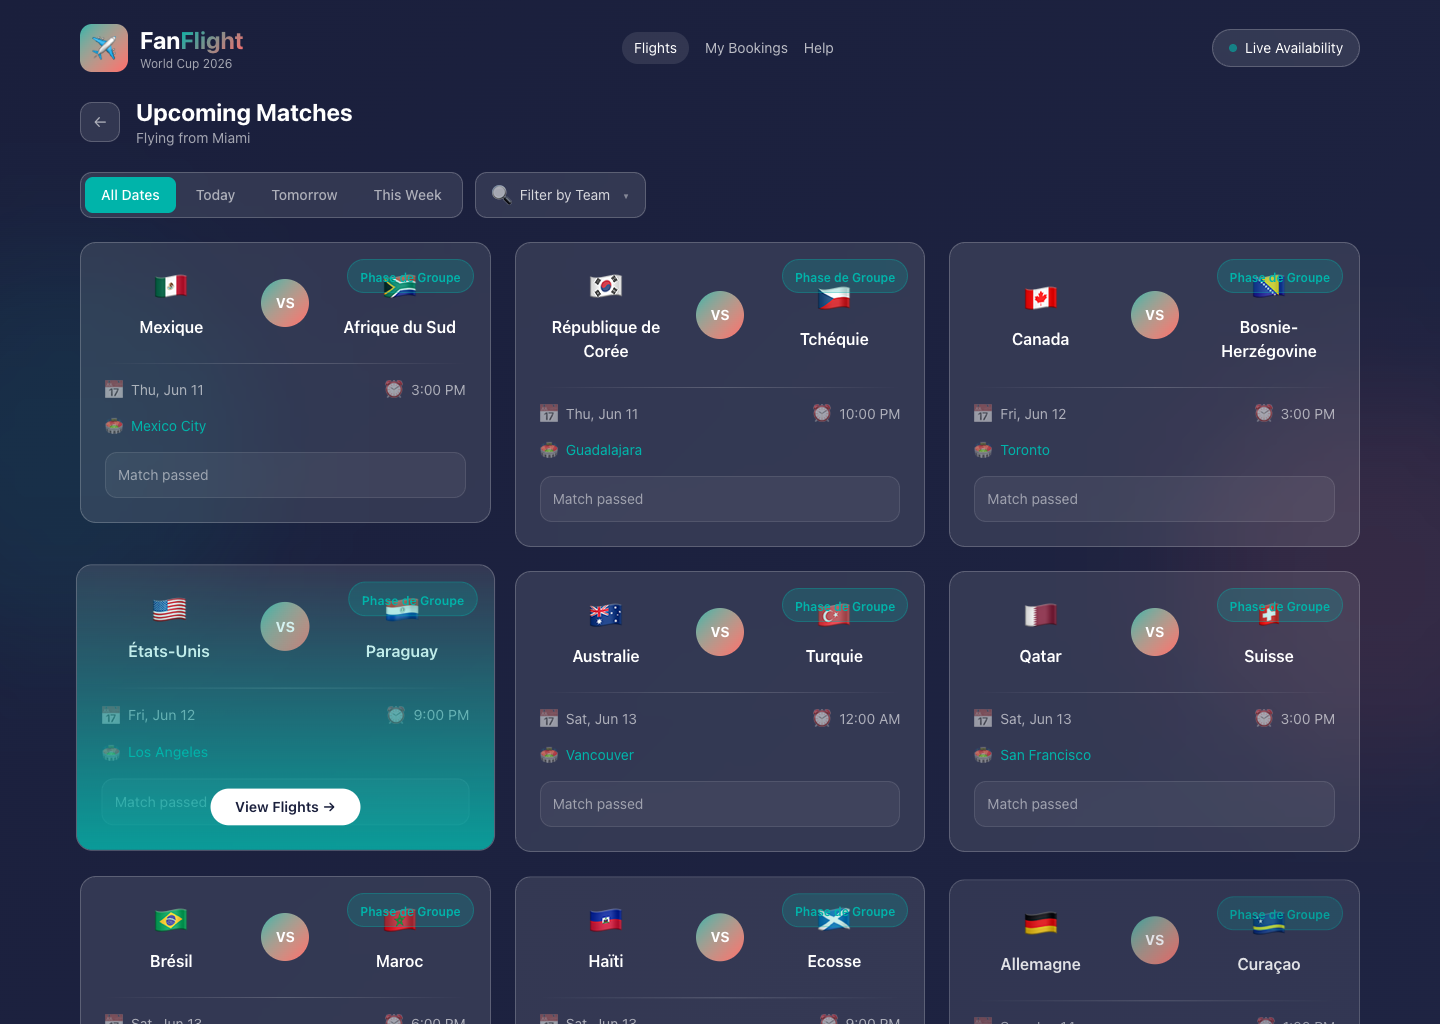
\includegraphics[width=0.9\textwidth]{img/app-matches-view.png}
\caption{Écran des matchs disponibles (\code{MatchFilters} + \code{MatchCard}) depuis Miami}
\label{fig:app-matches}
\end{figure}

L'interface repose sur Tailwind CSS 4 pour le style et ne nécessite aucune bibliothèque de gestion d'état externe, la complexité de l'application restant volontairement contenue pour un projet pédagogique mené à quatre.

\section{Conteneurisation et intégration/déploiement continus}

\subsection{Orchestration locale}

\begin{lstlisting}[caption={\code{docker-compose.yml} -- extrait, dépendances de démarrage}]
backend-api:
  build: ./API
  depends_on:
    db:
      condition: service_healthy

db:
  image: postgres:17
  healthcheck:
    test: ["CMD-SHELL", "pg_isready -U root -d ${DB_NAME}"]
\end{lstlisting}

L'image PostgreSQL est explicitement épinglée en version 17 plutôt que \code{latest} : un changement de version majeure non contrôlé pourrait rendre un volume de données existant incompatible sans migration explicite (\code{pg_upgrade}) -- un risque jugé inacceptable pour une base de production.

\subsection{Intégration continue : construction et publication des images}

Le workflow GitHub Actions \code{frontend-deploy.yml} se déclenche sur chaque \emph{push} vers la branche principale touchant le frontend, l'API ou le pipeline Spark, ou manuellement (\code{workflow_dispatch}). Il construit et publie trois images vers Docker Hub, chacune taguée à la fois \code{latest} et par le SHA du commit pour garantir la traçabilité :

\begin{lstlisting}[caption={Extrait du workflow -- publication taguée par SHA}]
- name: Build and push backend API image
  uses: docker/build-push-action@v6
  with:
    context: ./API
    tags: |
      ${{ env.BACKEND_API_IMAGE }}:latest
      ${{ env.BACKEND_API_IMAGE }}:${{ github.sha }}
\end{lstlisting}

\subsection{Déploiement continu : SSH, Docker Compose et Watchtower}

Le second job du workflow se connecte en SSH à l'instance de production, génère un fichier \code{docker-compose.yml} de production (ajoutant un service \code{watchtower} et des étiquettes \code{com.centurylinklabs.watchtower.enable=true} sur chaque service applicatif), puis démarre ou met à jour les services. Watchtower assure ensuite la mise à jour continue des conteneurs en production, en interrogeant Docker Hub toutes les 60 secondes, sans nouvelle intervention du pipeline CI :

\begin{lstlisting}[caption={Service Watchtower -- mise à jour continue en production}]
watchtower:
  image: containrrr/watchtower:latest
  command: --interval 60 --cleanup --label-enable
  volumes:
    - /var/run/docker.sock:/var/run/docker.sock
\end{lstlisting}

\section{Observabilité de l'infrastructure : Prometheus et Grafana}
\label{sec:monitoring}

\subsection{Présentation et objectif}

En complément du socle applicatif, Emy Regna a conçu et déployé, sur la même branche que l'extension machine learning, une chaîne d'observabilité complète de l'infrastructure FanFlight : supervision système, applicative et réseau, restituée dans un tableau de bord Grafana unique. Ce travail n'est pas encore fusionné dans la branche de production, mais démontre concrètement le volet « monitoring » de la compétence BC03 « Automatiser le déploiement de nouvelles versions de la solution et son monitoring ».

\subsection{Une chaîne de collecte à plusieurs niveaux}

La stack repose sur Prometheus comme collecteur central (scrutation toutes les 15 secondes), alimenté par cinq sources complémentaires, chacune couvrant un niveau différent de l'infrastructure :

\begin{itemize}
  \item \textbf{node-exporter} : métriques système de l'hôte (CPU, mémoire, disque) de l'instance EC2 de production ;
  \item \textbf{cAdvisor} : métriques par conteneur (CPU, mémoire), nécessitant un accès privilégié en lecture au socket Docker et au système de fichiers hôte ;
  \item \textbf{postgres-exporter} : métriques internes de la base PostgreSQL, connecté via la même chaîne de connexion applicative que l'API ;
  \item \textbf{Blackbox Exporter} : \emph{health-checks} HTTP actifs sur le frontend, la route \code{/ready} de l'API, et les interfaces web de Spark master et worker ;
  \item \textbf{Prometheus lui-même} : auto-supervision de sa propre disponibilité.
\end{itemize}

\begin{lstlisting}[caption={\code{monitoring/prometheus/prometheus.yml} -- health-checks HTTP via Blackbox Exporter}]
- job_name: service-health
  metrics_path: /probe
  params:
    module: [http_2xx]
  static_configs:
    - targets:
        - http://frontend:3000/
        - http://backend-api:8000/ready
        - http://spark-master:8080/
        - http://spark-worker:8081/
  relabel_configs:
    - source_labels: [__address__]
      target_label: __param_target
    - source_labels: [__param_target]
      target_label: instance
    - target_label: __address__
      replacement: blackbox-exporter:9115
\end{lstlisting}

Cette configuration illustre un motif classique de Blackbox Exporter : les cibles à sonder sont déclarées comme de simples URLs, puis réaffectées (\emph{relabeling}) pour être effectivement interrogées via l'exporter plutôt que directement -- Prometheus scrute ainsi la disponibilité de chaque service applicatif sans que celui-ci ait besoin d'exposer lui-même un point de métrique dédié.

\subsection{Restitution : un tableau de bord Grafana provisionné}

Grafana est connecté à Prometheus via une source de données provisionnée automatiquement au démarrage (fichier YAML, sans configuration manuelle dans l'interface), de même que le tableau de bord \emph{FanFlight Overview}, dont les sept panneaux couvrent les trois niveaux de supervision de la stack :

\begin{longtable}{p{4.2cm}p{4cm}p{5cm}}
\toprule
\textbf{Panneau} & \textbf{Niveau} & \textbf{Source} \\
\midrule
\endhead
Service Health Checks & Applicatif & Blackbox Exporter (\code{/probe}) \\
HTTP Probe Duration & Applicatif & Blackbox Exporter \\
Exporter Health & Infrastructure de monitoring & Prometheus (\emph{self-scrape} de chaque exporter) \\
EC2 CPU Usage & Système (hôte) & node-exporter \\
EC2 Memory Usage & Système (hôte) & node-exporter \\
EC2 Root Disk Usage & Système (hôte) & node-exporter \\
Container CPU Usage & Conteneur & cAdvisor \\
\bottomrule
\end{longtable}

\subsection{Intégration au déploiement}

La chaîne d'observabilité est packagée dans \code{docker-compose.local.yml} pour les tests, et son déploiement en production est intégré au workflow GitHub Actions : les fichiers de configuration sont copiés vers \code{/opt/fanflight/monitoring/} sur l'instance EC2, et les identifiants d'administration Grafana sont paramétrables par variable d'environnement plutôt que codés en dur. Comme pour l'extension machine learning, cette intégration n'est aujourd'hui présente que sur la branche de développement dédiée ; sa fusion vers la branche principale est identifiée comme une priorité de court terme (cf. section~\ref{sec:preconisations}).

\section{Extension Machine Learning : prédiction de retard de vol}
\label{sec:ml}

\subsection{Présentation et objectif}

En parallèle du socle décrit ci-dessus, Daniel Kouacou a développé, sur une branche dédiée du dépôt, une extension complète de machine learning visant à afficher, pour chaque vol proposé à un supporter, une probabilité de retard. Ce travail n'est pas encore fusionné dans la branche de production, mais constitue une démonstration à part entière de la compétence BC02 « développer un algorithme d'intelligence artificielle ».

\subsection{Un problème de cohérence des données résolu par une source alternative}

La première tentative de modélisation entraînait le modèle sur les vols 2026 renvoyés par SerpAPI, croisés avec une météo 2025 non alignée temporellement -- un défaut méthodologique documenté explicitement par son auteur. La solution retenue sépare proprement les deux flux :

\begin{itemize}
  \item \textbf{entraînement} : données réelles de ponctualité des vols domestiques américains publiées par le \emph{Bureau of Transportation Statistics} (BTS) pour mai, juin et juillet 2025, filtrées aux aéroports des villes hôtes de la Coupe du Monde, enrichies de la météo réelle du jour et de l'aéroport concernés (Open-Meteo) -- garantissant une cohérence temporelle complète entre le retard observé et la météo du jour ;
  \item \textbf{inférence} : les vols 2026 renvoyés par SerpAPI sont scorés en temps réel par le modèle ainsi entraîné, la météo utilisée à l'inférence provenant d'une prévision réelle si le vol a lieu dans les 16 jours, ou d'un repli saisonnier sinon.
\end{itemize}

\subsection{Un contrat de features partagé entre entraînement et inférence}

Pour éviter toute divergence entre les données vues à l'entraînement et celles vues en production (\emph{train/serve skew}), le module \code{feature_builder.py} (environ 165 lignes) est partagé entre le pipeline d'entraînement et l'API de service, garantissant un encodage strictement identique des 20 caractéristiques utilisées (horaires, durée, compagnie, aéroports, et sept variables météorologiques dont un score de risque dérivé du code météo).

\subsection{Entraînement, suivi et mise en service via MLflow}

Le script \code{train.py} (environ 440 lignes) entraîne et compare deux modèles -- XGBoost et un réseau de neurones PyTorch -- et journalise métriques, graphiques (SHAP, courbe ROC, matrice de confusion) et artefacts dans MLflow, avant de promouvoir le meilleur modèle au statut « Production » dans le registre de modèles. Au démarrage, l'API charge automatiquement la version la plus récente enregistrée dans le registre pour ce modèle -- qui correspond en pratique à la version promue, puisque chaque entraînement promeut la dernière version :

\begin{lstlisting}[language=Python, caption={Extrait de \code{main.py} (branche ML) -- chargement du modèle au démarrage}]
@app.on_event("startup")
def load_model():
    global MODEL, MAPPINGS, MODEL_NAME
    try:
        client = MlflowClient()
        versions = client.get_latest_versions("flight_delay_xgboost")
        latest = max(versions, key=lambda v: int(v.version))
        local_path = client.download_artifacts(latest.run_id, "model/model.xgb")
        booster = xgb.Booster()
        booster.load_model(local_path)
        MODEL = booster
    except Exception as e:
        print(f"[ML] Echec chargement XGBoost : {e}")
        print("[ML] API demarre sans modele - vols retournes sans score de retard.")
\end{lstlisting}

Ce chargement échoue de façon contrôlée -- l'API démarre sans modèle plutôt que de planter -- si aucun modèle n'a encore été entraîné et promu, ce qui constitue une limite assumée : le déploiement n'est pas encore auto-suffisant sans une exécution manuelle préalable du pipeline d'entraînement.

\subsection{Résultats et limites assumées}

Sur 628\,704 vols réels (contre 246 dans l'approche initiale fondée sur des données 2026 simulées), le taux de retard observé est de 27,8 \%, et le modèle XGBoost retenu atteint une AUC de 0,728 (contre 0,713 pour le réseau de neurones). Plusieurs limites sont explicitement documentées par l'auteur : le prix n'étant pas disponible dans les données BTS, cette variable est neutralisée à l'entraînement ; la durée de vol est approximée par la distance, faute de donnée directe ; et l'entraînement ne porte que sur des vols directs, les correspondances n'étant pas couvertes par le jeu de données BTS.

\subsection{Monitoring de dérive}

Le script \code{drift_monitor.py} (environ 355 lignes) compare la distribution des variables d'un nouveau lot de données à celle du jeu de référence via des tests statistiques (indice de stabilité de population -- PSI -- et test de Kolmogorov--Smirnov), posant les bases d'une supervision de la qualité du modèle en production dans la durée -- une pratique de MLOps mature, même si l'alerting automatique n'est pas encore implémenté.

\chapter{Description d'une situation de travail ayant nécessité une recherche}
\label{chap:recherche}

\section{Contexte de la problématique}

Dès la phase de conception de FanFlight, une contrainte s'est imposée comme structurante pour l'ensemble de l'architecture : l'API externe de vols (SerpAPI) facture chaque requête effectuée. Avec un budget personnel limité pour ce projet pédagogique, une architecture naïve -- interroger SerpAPI à chaque consultation d'un utilisateur, pour chaque combinaison de ville de départ et de match -- aurait rapidement épuisé notre quota, sans même garantir une expérience utilisateur rapide (chaque appel externe prenant plusieurs secondes).

Le problème à résoudre était donc double : ne jamais payer deux fois pour la même information, tout en construisant un système qui reste correct lorsque l'information n'est, par nature, pas immédiatement disponible sous une forme exploitable (une réponse SerpAPI est un document JSON complexe, pas une ligne de table prête à être filtrée en SQL).

\section{Démarche de recherche}

Plusieurs pistes ont été évaluées avant de converger vers la solution retenue :

\begin{itemize}
  \item \textbf{Cache côté frontend (navigateur)} : rejeté, car il ne mutualise rien entre utilisateurs différents interrogeant le même trajet, ce qui ne réduit pas le nombre d'appels à l'échelle de l'application ;
  \item \textbf{Cache mémoire côté API} : rejeté, car il serait perdu à chaque redémarrage de conteneur et ne serait pas partagé entre plusieurs instances de l'API si l'application devait être répliquée ;
  \item \textbf{Cache dédié (Redis)} : envisagé, mais écarté pour la durée du projet : il aurait ajouté un composant d'infrastructure supplémentaire à opérer et à sécuriser, pour un bénéfice marginal par rapport à une solution s'appuyant sur une base déjà présente dans l'architecture ;
  \item \textbf{Réutilisation de PostgreSQL comme cache durable} : retenue. La base de données, déjà nécessaire pour stocker le calendrier des matchs et les données de référence, pouvait aussi bien servir de mémoire persistante des résultats de vols déjà obtenus.
\end{itemize}

Cette dernière option soulevait cependant une difficulté : une réponse SerpAPI est un document JSON imbriqué, non directement interrogeable par une clause \code{WHERE} SQL utile (filtrer par ville, par date, par segment). Il fallait donc, en plus du cache lui-même, concevoir une étape de transformation entre la donnée brute reçue et la donnée requêtable.

\section{Implémentation de la solution}

La solution mise en œuvre combine trois éléments complémentaires :

\begin{enumerate}
  \item une table d'atterrissage \code{FLIGHTS_RAW} qui reçoit la réponse SerpAPI telle quelle, sous forme \code{JSONB}, sans bloquer sur sa transformation ;
  \item un pipeline de transformation asynchrone (Spark, déclenché par \code{LISTEN}/\code{NOTIFY}) qui structure cette donnée brute en lignes exploitables dans \code{FACT_FLIGHT}, sans quoi elle resterait inutilisable par une simple requête SQL ;
  \item une fonction de lecture (\code{check_flight_db}) systématiquement appelée \emph{avant} tout appel à SerpAPI, transformant l'appel externe en un recours de dernier ressort plutôt qu'un point de passage systématique.
\end{enumerate}

Un outil complémentaire, \code{replay_job.py}, exécuté automatiquement à chaque démarrage du conteneur API, permet de réinjecter dans le pipeline des réponses SerpAPI déjà obtenues et sauvegardées sur disque, sans consommer de nouveau quota d'API -- un choix directement motivé par la même contrainte de coût. Ce script n'est cependant pas idempotent : chaque redémarrage du conteneur déclenche un nouveau job de traitement, ce qui constitue une limite identifiée pour une exécution répétée en production (cf. section~\ref{sec:preconisations}).

\section{Itération ultérieure : un registre explicite des trajets déjà interrogés}

Le prolongement du projet par Daniel Kouacou (branche machine learning) a affiné cette stratégie de cache en documentant l'introduction d'une table \code{QUERIED_ROUTES}, destinée à enregistrer chaque trajet interrogé -- y compris lorsque SerpAPI n'a renvoyé \emph{aucun} vol -- avec un paramètre explicite (\code{force=true}) pour forcer un rafraîchissement volontaire (tests, données jugées obsolètes). Cette évolution, décrite dans la documentation du projet, corrige une limite identifiée de la première version : sans registre des trajets \emph{sans résultat}, un trajet effectivement sans vol disponible risquait d'être réinterrogé indéfiniment, consommant du quota pour ne jamais recevoir de réponse utile. À l'état actuel de la branche, cette table n'est cependant plus présente dans le code après une fusion intermédiaire ayant résolu \code{main.py} en faveur d'une autre branche parente -- un exemple concret de la difficulté à maintenir la cohérence entre documentation et code sur une branche de longue durée non encore intégrée à la production, et un point de vigilance retenu pour la fusion définitive de cette extension (cf. section~\ref{sec:preconisations}).

Cette itération illustre bien la nature incrémentale d'une problématique de coût en ingénierie de données : la première solution (cache positif via \code{FACT_FLIGHT}) a résolu le cas dominant, avant qu'un usage plus poussé du système ne révèle un angle mort (le cas négatif) que la solution suivante a cherché à traiter.

\chapter{Conclusion et ouverture}

\section{Synthèse du projet et réponse aux problématiques}

Le projet FanFlight visait à démontrer la maîtrise d'une démarche data engineering complète, de la modélisation des données jusqu'à la mise en production automatisée, au service d'un besoin concret : simplifier la planification de déplacements autour de la Coupe du Monde 2026. Au-delà de l'enjeu applicatif, l'objectif était de couvrir l'intégralité des compétences du référentiel RNCP38919 -- Data Engineer.

\textbf{Résultats obtenus :}
\begin{itemize}
  \item une application fonctionnelle en production, permettant de croiser calendrier de matchs et propositions de vols ;
  \item un modèle de données hybride (schéma en étoile + \code{JSONB}) adapté à une donnée externe volatile ;
  \item un pipeline ETL événementiel, idempotent, déclenché par notification PostgreSQL plutôt que par ordonnancement périodique ;
  \item une architecture explicitement conçue pour maîtriser le coût d'un service externe payant ;
  \item une chaîne CI/CD complète (GitHub Actions, Docker Hub, déploiement SSH, mise à jour continue par Watchtower) ;
  \item une chaîne d'observabilité de l'infrastructure (Prometheus, Grafana) couvrant les niveaux système, conteneur et applicatif ;
  \item une extension machine learning aboutie (XGBoost, MLflow, monitoring de dérive), démontrant la compétence d'intégration d'un algorithme d'intelligence artificielle dans une chaîne de données.
\end{itemize}

\section{Difficultés rencontrées et solutions apportées}

\textbf{Coût de l'API externe de vols.} SerpAPI facturant chaque requête, une architecture naïve n'était pas soutenable. \emph{Solution} : conception d'un cache durable porté par PostgreSQL, complété par un registre explicite des trajets déjà interrogés (cf. chapitre~\ref{chap:recherche}).

\textbf{Incertitude sur l'hébergement de production.} Aucune infrastructure de production n'était garantie au démarrage du projet. \emph{Solution} : développement et validation intégrale en local (Docker Compose) avant tout déploiement réel, ce qui a permis de ne pas bloquer l'avancement technique en attendant une solution d'hébergement ; celle-ci a finalement été apportée par notre école (Liora), qui a mis à disposition une instance AWS EC2 en fin de projet.

\textbf{Coordination d'une équipe distribuée et contrainte par des alternances.} Les quatre membres de l'équipe, répartis sur toute la France et engagés chacun dans une alternance en entreprise, ne pouvaient compter sur un temps de travail synchrone important. \emph{Solution} : discipline de revue de code asynchrone via des \emph{pull requests} GitHub, découpage du travail en lots intégrables indépendamment, et accompagnement régulier de notre mentor Dan Cohen pour garder le cap malgré l'absence de coprésence.

\section{Principaux bénéfices tirés du projet}

\textbf{Montée en compétences techniques :}
\begin{itemize}
  \item conception de modèles de données hybrides combinant schéma en étoile et données semi-structurées ;
  \item construction d'un pipeline de données événementiel avec Apache Spark et les primitives natives de PostgreSQL ;
  \item conteneurisation et automatisation complète d'une chaîne de déploiement (CI/CD, mise à jour continue) ;
  \item initiation concrète aux pratiques de MLOps (registre de modèles, monitoring de dérive) au travers de l'extension machine learning du projet.
\end{itemize}

\textbf{Compétences collectives :} la principale réussite de ce projet, au-delà de sa réalisation technique, a été de maintenir une collaboration efficace à quatre malgré nos contraintes organisationnelles (cf. chapitre~\ref{chap:cahier}) -- une compétence directement transférable à un contexte professionnel de travail distribué.

\section{Préconisations pour l'évolution du projet}
\label{sec:preconisations}

\textbf{Court terme :}
\begin{itemize}
  \item fusionner proprement l'extension machine learning et la chaîne d'observabilité Prometheus/Grafana dans la branche principale, en déplaçant les artefacts volumineux (jeux de données BTS, modèles) hors du dépôt Git vers un stockage dédié (versionnement de données, stockage objet), et en revalidant à cette occasion les fonctionnalités documentées mais perdues en cours de fusion (registre \code{QUERIED_ROUTES}) ;
  \item configurer des règles d'alerte Prometheus (Alertmanager) sur les métriques déjà collectées par Emy Regna (indisponibilité d'un service, saturation CPU/mémoire de l'instance EC2), pour transformer la supervision existante, aujourd'hui consultée manuellement dans Grafana, en une détection proactive des incidents ;
  \item remplacer l'attente synchrone de l'API pendant le traitement Spark par un mécanisme de notification asynchrone côté frontend, pour ne plus bloquer la requête HTTP jusqu'à 90 secondes ;
  \item rendre \code{replay_job.py} idempotent ou conditionnel à un premier démarrage, pour éviter de déclencher un nouveau job Spark à chaque redémarrage du conteneur API en production ;
  \item faire tourner les conteneurs API et Spark avec un utilisateur non privilégié, à l'image de ce qui est déjà fait pour le frontend ;
  \item ajouter la contrainte de clé étrangère entre \code{FACT_FLIGHT} et \code{DIM_AIRPORT} une fois \code{enrich_airports} déplacé avant le chargement des vols, pour que l'intégrité référentielle soit garantie par PostgreSQL plutôt que par la seule discipline applicative ;
  \item sécuriser les identifiants par défaut actuellement présents dans le code (mots de passe de secours codés en dur), au profit d'une gestion de secrets systématique.
\end{itemize}

\textbf{Moyen terme :}
\begin{itemize}
  \item mettre en place des tests automatisés (unitaires sur les fonctions de transformation, d'intégration sur le pipeline complet) dans la chaîne CI/CD ;
  \item ajouter un système d'alerte sur les résultats du monitoring de dérive du modèle de prédiction de retard ;
  \item implémenter le parcours de confirmation/réservation, aujourd'hui présent dans l'interface mais non connecté à une logique métier.
\end{itemize}

\textbf{Long terme :}
\begin{itemize}
  \item industrialiser le service du modèle de machine learning (service HTTP dédié plutôt que partage par volume Docker) ;
  \item étendre la couverture du calendrier aux phases finales de la compétition et généraliser le modèle de prédiction de retard au-delà des seuls vols directs.
\end{itemize}

\section{Ouverture}

Ce projet fil rouge a été, pour chacun des quatre membres de l'équipe, une mise en pratique concrète des compétences du métier de Data Engineer sur un cas d'usage complet -- de la modélisation d'un entrepôt de données jusqu'à l'intégration d'un modèle de machine learning en production. Les enseignements en dépassent le cadre pédagogique : la nécessité de concevoir une architecture de données sous contrainte de coût dès sa conception, l'exigence de rigueur qu'impose un pipeline automatisé et idempotent, et la capacité à faire fonctionner une équipe technique malgré la distance géographique sont autant de compétences que nous comptons chacun continuer à approfondir dans nos parcours respectifs en ingénierie des données -- que ce soit en consolidant nos pratiques d'architecture événementielle, en allant plus loin dans l'industrialisation de modèles de machine learning, ou en poursuivant l'exploration des pratiques de MLOps amorcées avec l'extension prédictive de FanFlight.

\chapter*{Annexes}
\addcontentsline{toc}{chapter}{Annexes}

\section*{Annexe A : Documentation officielle}
\addcontentsline{toc}{section}{Annexe A : Documentation officielle}

\textbf{FastAPI}
\begin{itemize}
  \item Documentation officielle : \url{https://fastapi.tiangolo.com/}
  \item Déploiement : \url{https://fastapi.tiangolo.com/deployment/}
\end{itemize}

\textbf{PostgreSQL}
\begin{itemize}
  \item Documentation officielle : \url{https://www.postgresql.org/docs/}
  \item LISTEN/NOTIFY : \url{https://www.postgresql.org/docs/current/sql-notify.html}
\end{itemize}

\textbf{Apache Spark / PySpark}
\begin{itemize}
  \item Documentation officielle : \url{https://spark.apache.org/docs/latest/api/python/}
  \item Spark SQL Functions : \url{https://spark.apache.org/docs/latest/api/python/reference/pyspark.sql/functions.html}
\end{itemize}

\textbf{Next.js}
\begin{itemize}
  \item Documentation officielle : \url{https://nextjs.org/docs}
\end{itemize}

\textbf{Docker et Docker Hub}
\begin{itemize}
  \item Documentation officielle Docker : \url{https://docs.docker.com/}
  \item Docker Compose : \url{https://docs.docker.com/compose/}
\end{itemize}

\textbf{GitHub Actions}
\begin{itemize}
  \item Documentation officielle : \url{https://docs.github.com/actions}
\end{itemize}

\textbf{MLflow}
\begin{itemize}
  \item Documentation officielle : \url{https://mlflow.org/docs/latest/index.html}
  \item Model Registry : \url{https://mlflow.org/docs/latest/model-registry.html}
\end{itemize}

\textbf{XGBoost}
\begin{itemize}
  \item Documentation officielle : \url{https://xgboost.readthedocs.io/}
\end{itemize}

\textbf{Observabilité (Prometheus, Grafana)}
\begin{itemize}
  \item Prometheus -- documentation officielle : \url{https://prometheus.io/docs/}
  \item Grafana -- documentation officielle : \url{https://grafana.com/docs/}
  \item Blackbox Exporter (health-checks HTTP) : \url{https://github.com/prometheus/blackbox_exporter}
  \item cAdvisor (métriques par conteneur) : \url{https://github.com/google/cadvisor}
\end{itemize}

\section*{Annexe B : Sources de données externes}
\addcontentsline{toc}{section}{Annexe B : Sources de données externes}

\begin{itemize}
  \item SerpAPI (Google Flights) : \url{https://serpapi.com/google-flights-api}
  \item Open-Meteo : \url{https://open-meteo.com/}
  \item Bureau of Transportation Statistics (BTS), On-Time Performance : \url{https://www.transtats.bts.gov/}
  \item FIFA -- Coupe du Monde 2026 : \url{https://www.fifa.com/fr/tournaments/mens/worldcup/canadamexicousa2026}
\end{itemize}

\section*{Annexe C : Blogs techniques et veille technologique}
\addcontentsline{toc}{section}{Annexe C : Blogs techniques et veille technologique}

\textbf{Ingénierie de données (blogs d'entreprise)}
\begin{itemize}
  \item AWS Big Data Blog : \url{https://aws.amazon.com/blogs/big-data/}
  \item Databricks Blog : \url{https://www.databricks.com/blog}
  \item Netflix Technology Blog : \url{https://netflixtechblog.com/}
  \item Uber Engineering Blog : \url{https://www.uber.com/blog/engineering/}
\end{itemize}

\textbf{Écosystème PostgreSQL et Python}
\begin{itemize}
  \item Planet PostgreSQL (agrégateur de blogs officiels) : \url{https://planet.postgresql.org/}
  \item Real Python (FastAPI, Python applicatif) : \url{https://realpython.com/}
\end{itemize}

\textbf{Architecture logicielle}
\begin{itemize}
  \item Martin Fowler -- articles sur les patterns de données et d'architecture : \url{https://martinfowler.com/}
\end{itemize}

\section*{Annexe D : Communautés et forums}
\addcontentsline{toc}{section}{Annexe D : Communautés et forums}

\textbf{Forums techniques}
\begin{itemize}
  \item Stack Overflow (tag \emph{apache-spark}) : \url{https://stackoverflow.com/questions/tagged/apache-spark}
  \item Stack Overflow (tag \emph{fastapi}) : \url{https://stackoverflow.com/questions/tagged/fastapi}
  \item Stack Overflow (tag \emph{postgresql}) : \url{https://stackoverflow.com/questions/tagged/postgresql}
  \item Stack Overflow (tag \emph{mlflow}) : \url{https://stackoverflow.com/questions/tagged/mlflow}
  \item Stack Overflow (tag \emph{grafana}) : \url{https://stackoverflow.com/questions/tagged/grafana}
\end{itemize}

\textbf{Reddit}
\begin{itemize}
  \item r/dataengineering : \url{https://www.reddit.com/r/dataengineering/}
  \item r/PostgreSQL : \url{https://www.reddit.com/r/PostgreSQL/}
  \item r/docker : \url{https://www.reddit.com/r/docker/}
\end{itemize}

\textbf{Slack et Discord}
\begin{itemize}
  \item MLOps Community Slack : \url{https://mlops.community/}
  \item dbt Community Slack (pratiques de transformation de données) : \url{https://www.getdbt.com/community/}
\end{itemize}

\textbf{GitHub Discussions}
\begin{itemize}
  \item Discussions des projets open-source mobilisés (FastAPI, Next.js, MLflow, Prometheus, Grafana)
\end{itemize}

\section*{Annexe E : Outils et utilitaires}
\addcontentsline{toc}{section}{Annexe E : Outils et utilitaires}

\begin{itemize}
  \item DBeaver / pgAdmin (exploration de la base PostgreSQL) : \url{https://dbeaver.io/}
  \item Docker Desktop (environnement de développement local) : \url{https://www.docker.com/products/docker-desktop/}
  \item Documentation OpenAPI interactive de FastAPI (\code{/docs}), pour tester l'API sans outil externe
  \item GitHub CLI (\code{gh}), pour piloter les \emph{pull requests} et les \emph{workflows} GitHub Actions en ligne de commande : \url{https://cli.github.com/}
  \item dbdiagram.io, pour esquisser et faire évoluer le schéma en étoile : \url{https://dbdiagram.io/}
\end{itemize}

\section*{Annexe F : Certifications et formations}
\addcontentsline{toc}{section}{Annexe F : Certifications et formations}

\begin{itemize}
  \item Fiche RNCP38919 -- Data engineer (France Compétences) : \url{https://www.francecompetences.fr/}
  \item DataScientest -- formation Data Engineer : \url{https://datascientest.com/data-engineer-rncp}
  \item AWS Certified Data Engineer -- Associate : \url{https://aws.amazon.com/certification/certified-data-engineer-associate/}
  \item Databricks Certified Data Engineer Associate : \url{https://www.databricks.com/learn/certification/data-engineer-associate}
\end{itemize}

\section*{Annexe G : Ressources complémentaires}
\addcontentsline{toc}{section}{Annexe G : Ressources complémentaires}

\textbf{Livres recommandés}
\begin{itemize}
  \item \emph{Fundamentals of Data Engineering} -- Joe Reis, Matt Housley (O'Reilly, 2022)
  \item \emph{Designing Data-Intensive Applications} -- Martin Kleppmann (O'Reilly, 2017)
  \item \emph{The Data Warehouse Toolkit} -- Ralph Kimball, Margy Ross -- référence directe pour la conception du schéma en étoile de FanFlight
\end{itemize}

\textbf{Podcasts}
\begin{itemize}
  \item Data Engineering Podcast (Tobias Macey) : \url{https://www.dataengineeringpodcast.com/}
  \item The Data Stack Show : \url{https://datastackshow.com/}
\end{itemize}

\textbf{Conférences}
\begin{itemize}
  \item Data Council : \url{https://www.datacouncil.ai/}
  \item dbt Coalesce (dbt Labs) : \url{https://coalesce.getdbt.com/}
\end{itemize}

\end{document}
